
\section*{CHƯƠNG 1. THU THẬP YÊU CẦU}
\setcounter{section}{1}
\setcounter{subsection}{0} %LƯU Ý MỖI LẦN THÊM CHƯƠNG MỚI CẦN THÊM CÂU NÀY ĐỂ RESET THỨ TỰ CỦA SUBSECTON VỀ 1
\setcounter{table}{0} % LƯU Ý SAU MỖI LẦN GỌI BẢNG HAY HÌNH ẢNH PHẢI THÊM CÂU NÀY ĐỂ RESET THỨ TỰ
\setcounter{figure}{0} %% LƯU Ý SAU MỖI LẦN GỌI BẢNG HAY HÌNH ẢNH PHẢI THÊM CÂU NÀY ĐỂ RESET THỨ TỰ
\addcontentsline{toc}{section}{\numberline{}CHƯƠNG 1. THU THẬP YÊU CẦU}
Chương này sẽ tiến hành thu thập yêu cầu cho dự án đề tài "Hệ thống theo dõi và quản lý dữ liệu điện tim" dựa trên các mục tiêu
đã nêu ra trong Mục Đề xuất hệ thống ở Phần mở đầu.

\subsection{Yêu cầu hệ thống}
\subsubsection{Yêu cầu về người dùng hệ thống}
Hệ thống được thiết kế để phục vụ các đối tượng sau:
\begin{adjustwidth}{1.5em}{}
\begin{itemize}
    \item Bệnh nhân: Người sử dụng hệ thống để thực hiện theo dõi dữ liệu điện tim thông qua website. Bệnh nhân có quyền truy cập vào kết quả ECG của mình, có thể được một bác sĩ phụ trách và theo dõi các thông tin liên quan đến điện tim và sức khoẻ
    \item Bác sĩ: Người sử dụng hệ thống để thực hiện quản lý, theo dõi các bệnh nhân mình được phân công. Bác sĩ có quyền truy cập vào kết quả ECG của bệnh nhân, có thể trao đổi, tư vấn với bệnh nhân về các thông tin liên quan
    \item Quản trị viên: Người sử dụng hệ thống để quản lý các tài khoản người dùng, thiết bị, quản lý phân công giữa bác sĩ và bệnh nhân, quản lý các bản dữ liệu đo
\end{itemize}
\end{adjustwidth}

\subsubsection{Yêu cầu chức năng}
Các chức năng chính của hệ thống bao gồm:
\begin{adjustwidth}{1.5em}{}
  \begin{itemize}
      \item Ghi lại dữ liệu thiết bị: Hệ thống cho phép ghi lại dữ liệu từ thiết bị y tế được truyền qua Mobile app. Dữ liệu được chuyển tới website của người dùng thông qua mobile app để lưu trữ, phân tích và có thể xem lại sau này
      \item Hiển thị và phân tích dữ liệu: Hệ thống hiển thị dữ liệu y tế theo dạng bảng biểu và đồ thị. Hệ thống cũng hỗ trợ xuất ra các tệp đã được chuẩn hoá cho các dữ liệu chuỗi thời gian (time-series database) để phục vụ mục đích phân tích và nghiên cứu
      \item Lưu trữ: Hệ thống hỗ trợ lưu dữ liệu mà người dùng đo được từ thiết bị trên cả ứng dụng và trên server của hệ thống. Dữ liệu điện tim cũng được đồng bộ hóa và lưu trữ trên máy chủ của hệ thống. Qua quá trình đồng bộ hóa, dữ liệu từ ứng dụng được truyền đến máy chủ và được lưu trữ an toàn và bảo mật trên hệ thống. Việc lưu trữ dữ liệu trên cả ứng dụng và máy chủ giúp đảm bảo rằng dữ liệu quan trọng này được lưu trữ một cách đáng tin cậy và có sẵn cho phân tích hoặc sử dụng tương lai
      \item Trao đổi và chia sẻ thông tin về dữ liệu y tế: Hệ thống giúp người dùng có thể trao đổi trực tiếp với bác sĩ và trợ lý ảo, chia sẻ kết quả đo điện tim, hỏi đáp về các vấn đề sức khỏe, các vấn đề liên quan đến hệ thống và thiết bị hoặc thảo luận về các quyết định. Điều này mang lại sự tiện lợi và hỗ trợ đáng kể cho người dùng trong việc xác định về tình trạng sức khoẻ hiện tại của bản thân.
      

  \end{itemize}
\end{adjustwidth}
% Hệ thống hỗ trợ các chức năng cơ bản sau đối với người dùng:
\textbf{Đối với bệnh nhân:}
\begin{adjustwidth}{1.5em}{}
\begin{itemize}
    \item Đăng nhập và đăng ký tài khoản bằng thông tin cá nhân, bao gồm tên, địa chỉ email, ngày sinh, số điện thoại và mật khẩu
    \item Cập nhật các thông tin cá nhân
    \item Được theo dõi điện tim trực tiếp khi kết nối ứng dụng di động với thiết bị đo điện tim thông qua Bluetooth
    \item Xem kết quả ECG của mình, bao gồm biểu đồ và các thông số liên quan
    \item Nhận thông báo và có thể trao đổi trực tiếp với bác sĩ về tình hình sức khoẻ và các kết quả đo được từ thiết bị
    \item Nhận tư vấn từ trợ lý ảo về hệ thống và các thông tin liên quan về sức khoẻ.
\end{itemize}
\end{adjustwidth}
\textbf{Đối với bác sĩ:}
\begin{adjustwidth}{1.5em}{}
\begin{itemize}
    \item Đăng nhập và đăng ký tài khoản bằng thông tin cá nhân, bao gồm tên, địa chỉ email, ngày sinh, số điện thoại và mật khẩu
    \item Cập nhật thông tin cá nhân
    \item Quản lý danh sách bệnh nhân
    \item Quản lý danh sách các bản ghi dữ liệu đo của các bệnh nhân trong list quản lý của mình
    \item Nhận thông báo và có thể trao đổi trực tiếp với bệnh nhân về tình hình sức khoẻ và các kết quả đo được từ thiết bị
    \item Tìm thêm thông tin về y tế và hệ thống này thông qua tương tác với trợ lý ảo 
\end{itemize}
\end{adjustwidth}
\textbf{Đối với quản trị viên:}
\begin{adjustwidth}{1.5em}{}
\begin{itemize}
    \item Đăng nhập và đăng ký tài khoản bằng thông tin cá nhân, bao gồm tên, địa chỉ email, số điện thoại và mật khẩu
    \item Cập nhật thông tin cá nhân
    \item Quản lý danh sách người dùng trong hệ thống, bao gồm bệnh nhân và bác sĩ
    \item Quản lý danh sách thiết bị, bản ghi của các dữ liệu
    \item Quản lý phân công bác sĩ - bệnh nhân
    \item Quản lý phê duyệt tài khoản khi người dùng đăng ký trên hệ thống
\end{itemize}
\end{adjustwidth}

\subsubsection{Yêu cầu phi chức năng}
\begin{itemize}
    \item Hệ thống hỗ trợ ngôn ngữ Tiếng Việt và Tiếng Anh
    \item Hệ thống có thể tương thích với hầu hết các trình duyệt phổ biến hiện nay
    \item Hệ thống đảm bảo tính bảo mật và quyền riêng tư thông tin của người dùng
    \item Hệ thống phải có giao diện người dùng thân thiện, dễ sử dụng để có thể tương tác mà không gặp quá nhiều khó khăn
    \item Thời gian phản hồi của hệ thống phải nhanh chóng và ổn định
    % \item Hệ thống cần sao lưu dữ liệu định kỳ để đảm bảo tính an toàn và khả năng khôi phục dữ liệu khi cần thiết.
\end{itemize}

% \subsection{Phân tích tổng quan hệ thống}
\subsection{Sơ đồ use case}
\subsubsection{Use case tổng quát hệ thống}
Dựa vào những phân tích về yêu cầu chức năng, các use case trong hệ thống được chúng em thể hiện ở hình dưới 

  \begin{figure}[H]
    \centering
    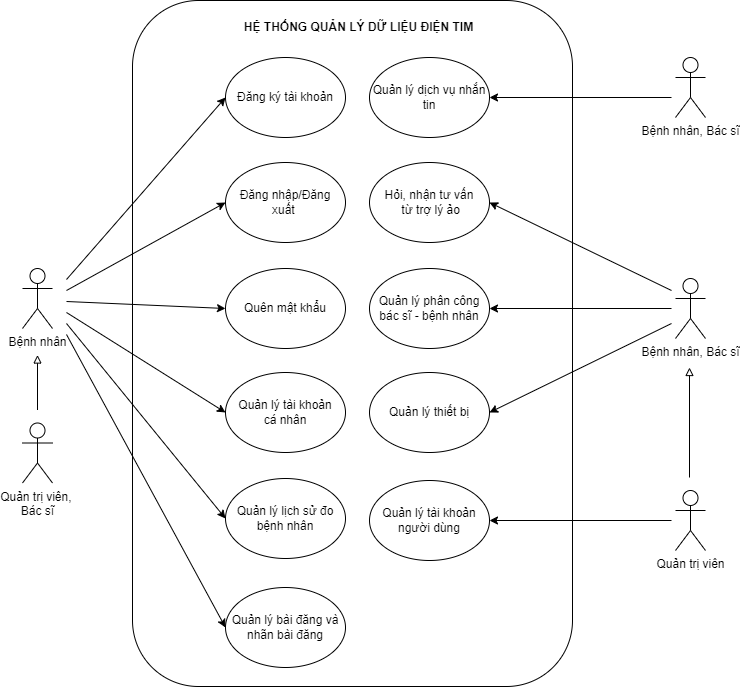
\includegraphics[width=16cm,height=14cm]{Images/use_case/use_case_general.png}
    \caption[Sơ đồ use case tổng quát của hệ thống]{\bfseries \fontsize{12pt}{0pt}
    \selectfont Sơ đồ use case tổng quát}
    \label{use_case_general} %đặt tên cho ảnh
  \end{figure}

\subsubsection{Use case đăng ký tài khoản}
  \begin{figure}[H]
    \centering
    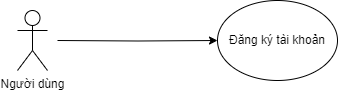
\includegraphics[width=9cm,height=2.5cm]{Images/use_case/use_case_register.png}
    \caption[Sơ đồ use case đăng ký tài khoản]{\bfseries \fontsize{12pt}{0pt}
    \selectfont Sơ đồ use case đăng ký tài khoản}
    \label{use_case_register} %đặt tên cho ảnh
  \end{figure}

  \begin{table}[H]
    \caption{\bfseries \fontsize{12pt}{0pt}\selectfont Bảng phân tích use case chức năng đăng ký tài khoản}
    \centering
    \begin{tabularx}{0.9\textwidth}{|c|X|}
      \hline
      \textbf{Tên chức năng} & \textbf{Đăng ký tài khoản} \\
      \hline
      Tác nhân & Bệnh nhân, Bác sĩ, Quản trị viên \\
      \hline
      Mô tả & Cho phép người dùng đăng ký tài khoản để truy cập vào các tài nguyên của hệ thống 
       \\
      \hline
      Điều kiện trước & Người dùng cần có kết nối Internet \\
      \hline
      Dòng sự kiện chính & 
      % \begin{tabular}{@{}l@{}}
        - Người dùng yêu cầu đăng ký tài khoản

        - Người dùng cung cấp thông tin tài khoản để đăng ký

        - Hệ thống xác minh các thông tin, nếu thỏa mãn sẽ thông báo thành công và kết thúc luồng sự kiện, ngược lại 
        sẽ thông báo lỗi 
        \\
      % \end{tabular} \\
      \hline
    \end{tabularx}
  \end{table}

\subsubsection{Use case chức năng đăng nhập/đăng xuất}
  \begin{figure}[H]
    \centering
    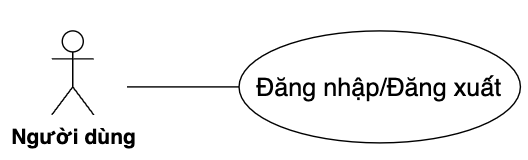
\includegraphics[width=9cm,height=2.5cm]{Images/use_case/use_case_login.png}
    \caption[Sơ đồ use case chức năng đăng nhập/đăng xuất]{\bfseries \fontsize{12pt}{0pt}
    \selectfont Sơ đồ use case chức năng đăng nhập/đăng xuất}
    \label{use_case_login_logout} %đặt tên cho ảnh
  \end{figure}

  \begin{table}[H]
    \caption{\bfseries \fontsize{12pt}{0pt}\selectfont Bảng phân tích use case chức năng đăng nhập/đăng xuất}
    \centering
    \begin{tabularx}{0.9\textwidth}{|c|X|}
      \hline
      \textbf{Tên chức năng} & \textbf{Đăng nhập/Đăng xuất} \\
      \hline
      Tác nhân & Bệnh nhân, Bác sĩ, Quản trị viên \\
      \hline
      Mô tả & Cho phép người dùng sử dụng tài khoản để truy cập vào các tài nguyên của hệ thống và có thể đăng xuất hệ thống
       \\
      \hline
      Điều kiện trước & Người dùng cần có kết nối Internet \\
      \hline
      Dòng sự kiện chính & 
      % \begin{tabular}{@{}l@{}}
        Chức năng đăng nhập:

        - Người dùng yêu cầu đăng nhập

        - Người dùng cung cấp thông tin đăng nhập

        - Hệ thống xác minh các thông tin, nếu thỏa mãn sẽ thông báo thành công và kết thúc luồng sự kiện, ngược lại 
        sẽ thông báo lỗi 

        Chức năng đăng xuất:

        - Người dùng yêu cầu đăng xuất

        - Hệ thống đăng xuất tài khoản người dùng và kết thúc luồng sự kiện
        \\
      % \end{tabular} \\
      \hline
    \end{tabularx}
  \end{table}

\subsubsection{Use case chức năng quên mật khẩu}
  \begin{figure}[H]
    \centering
    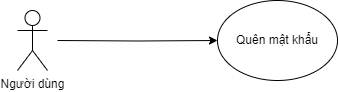
\includegraphics[width=9cm,height=2.5cm]{Images/use_case/use_case_forgot_password.png}
    \caption[Sơ đồ use case chức năng quên mật khẩu]{\bfseries \fontsize{12pt}{0pt}
    \selectfont Sơ đồ use case chức năng quên mật khẩu}
    \label{use_case_forget_password} %đặt tên cho ảnh
  \end{figure}

  \begin{table}[H]
    \caption{\bfseries \fontsize{12pt}{0pt}\selectfont Bảng phân tích use case chức năng quên mật khẩu}
    \centering
    \begin{tabularx}{0.9\textwidth}{|c|X|}
      \hline
      \textbf{Tên chức năng} & \textbf{Quên mật khẩu} \\
      \hline
      Tác nhân & Bệnh nhân, Bác sĩ, Quản trị viên \\
      \hline
      Mô tả & Cho phép người dùng lấy lại mật khẩu tài khoản thông qua email
       \\
      \hline
      Điều kiện trước & Người dùng cần có kết nối Internet và truy cập vào email đăng ký \\
      \hline
      Dòng sự kiện chính & 
      % \begin{tabular}{@{}l@{}}
        - Người dùng yêu cầu quên mật khẩu

        - Người dùng cung cấp email tài khoản để xác nhận

        - Hệ thống xác minh các thông tin, nếu thỏa mãn sẽ thông báo thành công và yêu cầu người dùng cung cấp mật khẩu mới, ngược lại 
        sẽ thông báo lỗi 


        - Hệ thống xác minh các thông tin, nếu thỏa mãn sẽ thông báo thành công và kết thúc luồng sự kiện, ngược lại 
        sẽ thông báo lỗi 
        \\
      % \end{tabular} \\
      \hline
    \end{tabularx}
  \end{table}

\subsubsection{Use case chức năng quản lý tài khoản cá nhân}
  \begin{figure}[H]
    \centering
    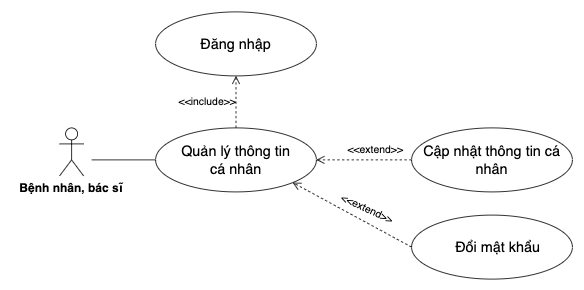
\includegraphics[width=12cm,height=6cm]{Images/use_case/use_case_manage_info.png}
    \caption[Sơ đồ use case chức năng quản lý tài khoản cá nhân]{\bfseries \fontsize{12pt}{0pt}
    \selectfont Sơ đồ use case chức năng quản lý tài khoản cá nhân}
    \label{use_case_manage_info} %đặt tên cho ảnh
  \end{figure}

  \begin{table}[H]
    \caption{\bfseries \fontsize{12pt}{0pt}\selectfont Bảng phân tích use case chức năng quản lý tài khoản cá nhân}
    \centering
    \begin{tabularx}{0.9\textwidth}{|c|X|}
      \hline
      \textbf{Tên chức năng} & \textbf{Quản lý tài khoản cá nhân} \\
      \hline
      Tác nhân & Bệnh nhân, Bác sĩ, Quản trị viên \\
      \hline
      Mô tả & Cho phép người dùng xem, thay đổi thông tin cá nhân trong tài khoản người dùng
       \\
      \hline
      Điều kiện trước & Người dùng cần có kết nối Internet và đăng nhập \\
      \hline
      Dòng sự kiện chính & 
      % \begin{tabular}{@{}l@{}}
        - Người dùng yêu cầu cập nhật thông tin cá nhân

        - Hệ thống cung cấp thông tin cá nhân của người dùng

        - Người dùng cung cấp thông tin cập nhật ài khoản cho hệ thống

        - Hệ thống xác minh các thông tin, nếu thỏa mãn sẽ thông báo thành công và kết thúc luồng sự kiện, ngược lại 
        sẽ thông báo lỗi         
        \\
      % \end{tabular} \\
      \hline
    \end{tabularx}
  \end{table}

\subsubsection{Use case chức năng quản lý lịch sử đo bệnh nhân}
  \begin{figure}[H]
    \centering
    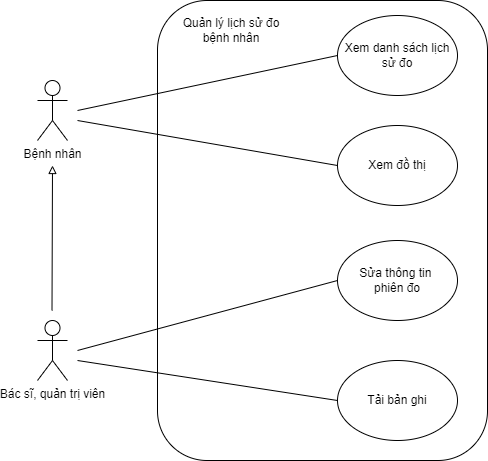
\includegraphics[width=12cm,height=11cm]{Images/use_case/use_case_view_history_record.png}
    \caption[Sơ đồ use case chức năng quản lý lịch sử đo bệnh nhân]{\bfseries \fontsize{12pt}{0pt}
    \selectfont Sơ đồ use case chức năng quản lý lịch sử đo bệnh nhân}
    \label{use_case_view_history_record} %đặt tên cho ảnh
  \end{figure}

  \begin{table}[H]
    \caption{\bfseries \fontsize{12pt}{0pt}\selectfont Bảng phân tích use case chức năng xem danh sách lịch sử phiên đo}
    \centering
    \begin{tabularx}{0.9\textwidth}{|c|X|}
      \hline
      \textbf{Tên chức năng} & \textbf{Xem danh sách lịch sử phiên đo} \\
      \hline
      Tác nhân & Bệnh nhân, Bác sĩ, Quản trị viên \\
      \hline
      Mô tả & Cho phép bệnh nhân xem lịch sử các phiên đo, bác sĩ xem được lịch sử các lần đo của bệnh nhân
      mà mình quản lý.\\
      \hline
      Điều kiện trước & Người dùng cần có kết nối Internet và đã đăng nhập \\
      \hline
      Dòng sự kiện chính & 
      % \begin{tabular}{@{}l@{}}
        - Người dùng yêu cầu quản lý lịch sử đo bệnh nhân

        - Hệ thống cung cấp danh sách phiên đo của người dùng (đối với bệnh nhân), danh sách phiên đo của 
        bệnh nhân mà bác sĩ phụ trách (đối với bác sĩ), danh sách tất cả phiên đo (đối với quản trị viên). Luồng sự kiện 
        kết thúc
        \\
      % \end{tabular} \\
      \hline
    \end{tabularx}
  \end{table}

  \begin{table}[H]
    \caption{\bfseries \fontsize{12pt}{0pt}\selectfont Bảng phân tích use case chức năng xem đồ thị}
    \centering
    \begin{tabularx}{0.9\textwidth}{|c|X|}
      \hline
      \textbf{Tên chức năng} & \textbf{Xem đồ thị} \\
      \hline
      Tác nhân & Bệnh nhân, Bác sĩ, Quản trị viên \\
      \hline
      Mô tả & Cho phép bệnh nhân xem đồ thị trong lần đo điện tim, bác sĩ xem được đồ thị của bệnh nhân
      mà mình quản lý.\\
      \hline
      Điều kiện trước & Người dùng cần có kết nối Internet và đã đăng nhập \\
      \hline
      Dòng sự kiện chính & 
      % \begin{tabular}{@{}l@{}}
        - Người dùng yêu cầu xem một phiên đo bất kì

        - Hệ thống cung cấp đồ thị dựa trên dữ liệu phiên đo mà người dùng đã yêu cầu, luồng sự kiện 
        kết thúc        
        \\
      % \end{tabular} \\
      \hline
    \end{tabularx}
  \end{table}
  \begin{table}[H]
    \caption{\bfseries \fontsize{12pt}{0pt}\selectfont Bảng phân tích use case chức năng sửa thông tin phiên đo}
    \centering
    \begin{tabularx}{0.9\textwidth}{|c|X|}
      \hline
      \textbf{Tên chức năng} & \textbf{Sửa thông tin phiên đo} \\
      \hline
      Tác nhân & Bác sĩ, Quản trị viên \\
      \hline
      Mô tả & Cho phép bác sĩ sửa thông tin phiên đo đo của bệnh nhân
      mà mình quản lý, quản trị viên có thể sửa thông tin phiên đo bất kì.\\
      \hline
      Điều kiện trước & Người dùng cần có kết nối Internet và đã đăng nhập \\
      \hline
      Dòng sự kiện chính & 
      % \begin{tabular}{@{}l@{}}
        - Bác sĩ, Quản trị viên yêu cầu cập nhật thông tin phiên đo

        - Hệ thống cung cấp thông tin phiên đo

        - Bác sĩ, Quản trị viên cung cấp thông tin cập nhật cho hệ thống

        - Hệ thống xác minh các thông tin, nếu thỏa mãn sẽ thông báo thành công và kết thúc luồng sự kiện, ngược lại 
        sẽ thông báo lỗi          
        \\
      % \end{tabular} \\
      \hline
    \end{tabularx}
  \end{table}

  \begin{table}[H]
    \caption{\bfseries \fontsize{12pt}{0pt}\selectfont Bảng phân tích use case chức năng tải bản ghi dữ liệu đo}
    \centering
    \begin{tabularx}{0.9\textwidth}{|c|X|}
      \hline
      \textbf{Tên chức năng} & \textbf{Tải bản ghi dữ liệu đo} \\
      \hline
      Tác nhân & Bác sĩ, Quản trị viên \\
      \hline
      Mô tả & Cho phép bác sĩ tải bản ghi dữ liệu đo của bệnh nhân
      mà mình quản lý, quản trị viên có thể tải bản đo dữ liệu bất kì.\\
      \hline
      Điều kiện trước & Người dùng cần có kết nối Internet và đã đăng nhập \\
      \hline
      Dòng sự kiện chính & 
      % \begin{tabular}{@{}l@{}}
        - Người dùng yêu cầu tải bản ghi dữ liệu

        - Hệ thống trả về tệp dữ liệu phiên đo, luồng sự kiện kết thúc        
        \\
      % \end{tabular} \\
      \hline
    \end{tabularx}
  \end{table}

\subsubsection{Use case chức năng quản lý dịch vụ nhắn tin}
  \begin{figure}[H]
    \centering
    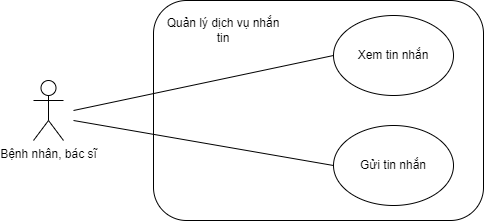
\includegraphics[width=12cm,height=6cm]{Images/use_case/use_case_send_receive_message.png}
    \caption[Sơ đồ use case chức năng quản lí dịch vụ nhắn tin]{\bfseries \fontsize{12pt}{0pt}
    \selectfont Sơ đồ use case chức năng quản lí dịch vụ nhắn tin}
    \label{use_case_chat} %đặt tên cho ảnh
  \end{figure}

  \begin{table}[H]
    \caption{\bfseries \fontsize{12pt}{0pt}\selectfont Bảng phân tích use case chức năng quản lí dịch vụ nhắn tin}
    \centering
    \begin{tabularx}{0.9\textwidth}{|c|X|}
      \hline
      \textbf{Tên chức năng} & \textbf{Xem/Gửi tin nhắn} \\
      \hline
      Tác nhân & Bệnh nhân, Bác sĩ \\
      \hline
      Mô tả & Cho phép bệnh nhân chat với bác sĩ phụ trách và bác sĩ có thể chat với bệnh nhân mà mình phụ trách \\
      \hline
      Điều kiện trước & Người dùng cần có kết nối Internet và đã đăng nhập \\
      \hline
      Dòng sự kiện chính & 
      % \begin{tabular}{@{}l@{}}
        - Bệnh nhân, Bác sĩ yêu cầu nhắn tin với bệnh nhân

        - Hệ thống cung cấp lịch sử cuộc hội thoại

        - Bệnh nhân, Bác sĩ trao đổi tin nhắn. Luồng sự kiện kết thúc
        \\
      % \end{tabular} \\
      \hline
    \end{tabularx}
  \end{table}

\subsubsection{Use case chức năng hỏi, nhận tư vấn từ trợ lý ảo}
  \begin{figure}[H]
    \centering
    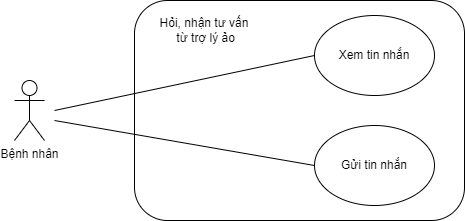
\includegraphics[width=12cm,height=6cm]{Images/use_case/use_case_chatbot.png}
    \caption[Sơ đồ use case chức năng hỏi, nhận tư vấn từ trợ lý ảo]{\bfseries \fontsize{12pt}{0pt}
    \selectfont Sơ đồ use case chức năng hỏi, nhận tư vấn từ trợ lý ảo}
    \label{use_case_chat_ai} %đặt tên cho ảnh
  \end{figure}
  \begin{table}[H]
    \caption{\bfseries \fontsize{12pt}{0pt}\selectfont Bảng phân tích use case chức năng gửi tin nhắn cho trợ lý ảo}
    \centering
    \begin{tabularx}{0.9\textwidth}{|c|X|}
      \hline
      \textbf{Tên chức năng} & \textbf{Xem/Gửi tin nhắn cho trợ lý ảo} \\
      \hline
      Tác nhân & Bệnh nhân \\
      \hline
      Mô tả & Cho phép bệnh nhân gửi câu hỏi và nhận tư vấn từ chat bot trợ lý ảo \\
      \hline
      Điều kiện trước & Người dùng cần có kết nối Internet và đã đăng nhập \\
      \hline
      Dòng sự kiện chính & 
      % \begin{tabular}{@{}l@{}}
        - Người dùng yêu cầu hỏi, nhận tư vấn từ trợ lý ảo
        
        - Người dùng cung cấp tin nhắn và gửi tới trợ lý ảo 

        - Sau đó, trợ lý ảo sẽ phản hồi lại tin nhắn và hiện phản hồi lên màn hình. Luồng sự kiện kết thúc
        \\
      % \end{tabular} \\
      \hline
    \end{tabularx}
  \end{table}  

  \subsubsection{Use case chức năng quản lý phân công bác sĩ - bệnh nhân}
  \begin{figure}[H]
    \centering
    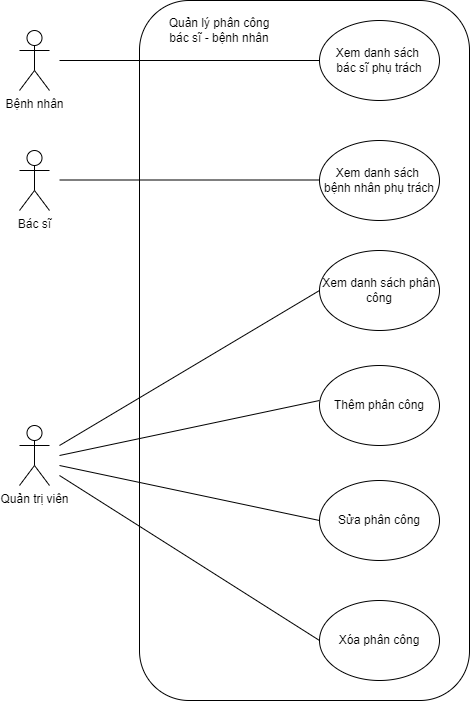
\includegraphics[width=12cm,height=16cm]{Images/use_case/use_case_manage_pda.png}
    \caption[Sơ đồ use case chức năng quản lý phân công bác sĩ - bệnh nhân]{\bfseries \fontsize{12pt}{0pt}
    \selectfont Sơ đồ use case chức năng quản lý phân công bác sĩ - bệnh nhân}
    \label{use_case_pda_management} %đặt tên cho ảnh
  \end{figure}

  \begin{table}[H]
    \caption{\bfseries \fontsize{12pt}{0pt}\selectfont Bảng phân tích use case chức năng xem danh sách bác sĩ}
    \centering
    \begin{tabularx}{0.9\textwidth}{|c|X|}
      \hline
      \textbf{Tên chức năng} & \textbf{Xem danh sách bác sĩ} \\
      \hline
      Tác nhân & Bệnh nhân \\
      \hline
      Mô tả & Cho phép bệnh nhân thực hiện hành động xem danh sách bác sĩ phụ trách mình \\
      \hline
      Điều kiện trước & Người dùng cần có kết nối Internet và đã đăng nhập \\
      \hline
      Dòng sự kiện chính & 
      % \begin{tabular}{@{}l@{}}
        - Bệnh nhân yêu cầu xem danh sách bác sĩ
        
        - Hệ thống cung cấp danh sách bác sĩ phụ trách bệnh nhân. Luồng sự kiện kết thúc        
        \\
      % \end{tabular} \\
      \hline
    \end{tabularx}
  \end{table}

  \begin{table}[H]
    \caption{\bfseries \fontsize{12pt}{0pt}\selectfont Bảng phân tích use case chức năng xem danh sách bệnh nhân}
    \centering
    \begin{tabularx}{0.9\textwidth}{|c|X|}
      \hline
      \textbf{Tên chức năng} & \textbf{Xem danh sách bệnh nhân} \\
      \hline
      Tác nhân & Bác sĩ \\
      \hline
      Mô tả & Cho phép bác sĩ thực hiện hành động xem danh sách bệnh nhân của mình \\
      \hline
      Điều kiện trước & Người dùng cần có kết nối Internet và đã đăng nhập \\
      \hline
      Dòng sự kiện chính & 
      % \begin{tabular}{@{}l@{}}
        - Bác sĩ yêu cầu xem danh sách bệnh nhân
        
        - Hệ thống cung cấp danh sách bệnh nhân mà bác sĩ phụ trách. Luồng sự kiện kết thúc         
        \\
      % \end{tabular} \\
      \hline
    \end{tabularx}
  \end{table}
  
  \begin{table}[H]
    \caption{\bfseries \fontsize{12pt}{0pt}\selectfont Bảng phân tích use case chức năng xem danh sách phân công bác sĩ - bệnh nhân}
    \centering
    \begin{tabularx}{0.9\textwidth}{|c|X|}
      \hline
      \textbf{Tên chức năng} & \textbf{Xem danh sách phân công bác sĩ - bệnh nhân} \\
      \hline
      Tác nhân & Quản trị viên \\
      \hline
      Mô tả & Cho phép quản trị thực hiện hành động xem danh sách phân công bác sĩ - bệnh nhân \\
      \hline
      Điều kiện trước & Người dùng cần có kết nối Internet và đã đăng nhập \\
      \hline
      Dòng sự kiện chính & 
      % \begin{tabular}{@{}l@{}}
        - Quản trị viên yêu cầu xem danh sách phân công bác sĩ - bệnh nhân
        
        - Hệ thống cung cấp danh sách phân công, luồng sự kiện kết thúc         
        \\
      % \end{tabular} \\
      \hline
    \end{tabularx}
  \end{table}

  \begin{table}[H]
    \caption{\bfseries \fontsize{12pt}{0pt}\selectfont Bảng phân tích use case chức năng thêm phân công bác sĩ - bệnh nhân}
    \centering
    \begin{tabularx}{0.9\textwidth}{|c|X|}
      \hline
      \textbf{Tên chức năng} & \textbf{Thêm phân công bác sĩ - bệnh nhân} \\
      \hline
      Tác nhân & Quản trị viên \\
      \hline
      Mô tả & Cho phép quản trị viên thực hiện hành động thêm phân công bác sĩ - bệnh nhân \\
      \hline
      Điều kiện trước & Người dùng cần có kết nối Internet và đã đăng nhập \\
      \hline
      Dòng sự kiện chính & 
      % \begin{tabular}{@{}l@{}}
        - Quản trị viên yêu cầu thêm phân công bác sĩ - bệnh nhân

        - Quản trị viên cung cấp thông tin phân công

        - Hệ thống xác minh các thông tin, nếu thỏa mãn sẽ thông báo thành công và kết thúc luồng sự kiện, ngược lại 
        sẽ thông báo lỗi         
        \\
      % \end{tabular} \\
      \hline
    \end{tabularx}
  \end{table}

  \begin{table}[H]
    \caption{\bfseries \fontsize{12pt}{0pt}\selectfont Bảng phân tích use case chức năng sửa thông tin phân công bác sĩ - bệnh nhân}
    \centering
    \begin{tabularx}{0.9\textwidth}{|c|X|}
      \hline
      \textbf{Tên chức năng} & \textbf{Sửa thông tin phân công bác sĩ - bệnh nhân} \\
      \hline
      Tác nhân & Quản trị viên \\
      \hline
      Mô tả & Cho phép quản trị viên thực hiện hành động sửa thông tin phân công bác sĩ - bệnh nhân \\
      \hline
      Điều kiện trước & Người dùng cần có kết nối Internet và đã đăng nhập \\
      \hline
      Dòng sự kiện chính & 
      % \begin{tabular}{@{}l@{}}
        - Quản trị viên yêu cầu cập nhật thông tin phân công bác sĩ - bệnh nhân

        - Quản trị viên cung cấp thông tin cập nhật trên màn hình và nhấn xác nhận

        - Hệ thống xác minh các thông tin, nếu thỏa mãn sẽ thông báo thành công và kết thúc luồng sự kiện, ngược lại 
        sẽ thông báo lỗi         
        \\
      % \end{tabular} \\
      \hline
    \end{tabularx}
  \end{table}

  \begin{table}[H]
    \caption{\bfseries \fontsize{12pt}{0pt}\selectfont Bảng phân tích use case chức năng xóa phân công bác sĩ - bệnh nhân}
    \centering
    \begin{tabularx}{0.9\textwidth}{|c|X|}
      \hline
      \textbf{Tên chức năng} & \textbf{Xóa phân công bác sĩ - bệnh nhân} \\
      \hline
      Tác nhân & Quản trị viên \\
      \hline
      Mô tả & Cho phép quản trị viên thực hiện hành động xóa phân công bác sĩ - bệnh nhân \\
      \hline
      Điều kiện trước & Người dùng cần có kết nối Internet và đã đăng nhập \\
      \hline
      Dòng sự kiện chính & 
      % \begin{tabular}{@{}l@{}}
        - Quản trị viên chọn một hoặc nhiều phân công và nhấn nút xóa

        - Hệ thống hiển thị màn xác nhận xóa

        - Quản trị viên chọn xác nhận xóa, hệ thống xóa thông tin và gửi thông báo kết quả. Ngược lại, quản trị viên 
        chọn hủy bỏ, hệ thống sẽ quay về màn danh sách phân công. Luồng sự kiện kết thúc
        \\
      % \end{tabular} \\
      \hline
    \end{tabularx}
  \end{table}

\subsubsection{Use case chức năng quản lý thiết bị}
  \begin{figure}[H]
    \centering
    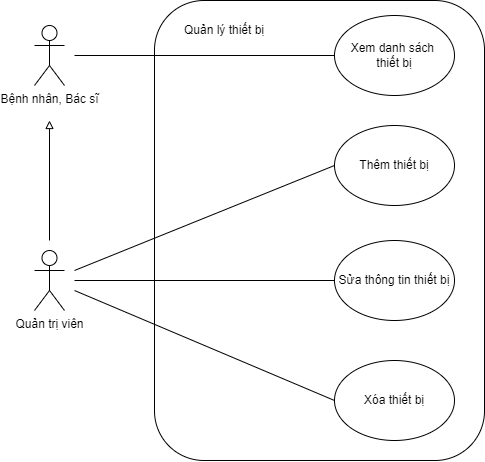
\includegraphics[width=12cm,height=11cm]{Images/use_case/use_case_manage_device.png}
    \caption[Sơ đồ use case chức năng quản lý thiết bị]{\bfseries \fontsize{12pt}{0pt}
    \selectfont Sơ đồ use case chức năng quản lý thiết bị}
    \label{use_case_device_management} %đặt tên cho ảnh
  \end{figure}

  \begin{table}[H]
    \caption{\bfseries \fontsize{12pt}{0pt}\selectfont Bảng phân tích use case chức năng xem danh sách thiết bị}
    \centering
    \begin{tabularx}{0.9\textwidth}{|c|X|}
      \hline
      \textbf{Tên chức năng} & \textbf{Xem danh sách thiết bị} \\
      \hline
      Tác nhân & Bệnh nhân, Bác sĩ, Quản trị viên \\
      \hline
      Mô tả & Cho phép quản trị viên thực hiện hành động xem thông tin danh sách thiết bị \\
      \hline
      Điều kiện trước & Người dùng cần có kết nối Internet và đã đăng nhập \\
      \hline
      Dòng sự kiện chính & 
      % \begin{tabular}{@{}l@{}}
        - Người dùng yêu cầu xem danh sách thiết bị
        
        - Hệ thống cung cấp danh sách thiết bị sử dụng (đối với bệnh nhân), danh sách thiết bị bác sĩ phụ trách (đối với bác sĩ), 
        danh sách tất cả thiết bị (đối với quản trị viên). Luồng sự kiện kết thúc 
        \\
      % \end{tabular} \\
      \hline
    \end{tabularx}
  \end{table}

  \begin{table}[H]
    \caption{\bfseries \fontsize{12pt}{0pt}\selectfont Bảng phân tích use case chức năng thêm thiết bị}
    \centering
    \begin{tabularx}{0.9\textwidth}{|c|X|}
      \hline
      \textbf{Tên chức năng} & \textbf{Thêm thiết bị} \\
      \hline
      Tác nhân & Quản trị viên \\
      \hline
      Mô tả & Cho phép quản trị viên thực hiện hành động thêm thiết bị vào danh sách thiết bị\\
      \hline
      Điều kiện trước & Người dùng cần có kết nối Internet và đã đăng nhập \\
      \hline
      Dòng sự kiện chính & 
      % \begin{tabular}{@{}l@{}}
        - Quản trị viên yêu cầu thêm thiết bị

        - Quản trị viên cung cấp thông tin thiết bị

        - Hệ thống xác minh các thông tin, nếu thỏa mãn sẽ thông báo thành công và kết thúc luồng sự kiện, ngược lại 
        sẽ thông báo lỗi           
        \\
      % \end{tabular} \\
      \hline
    \end{tabularx}
  \end{table}

  \begin{table}[H]
    \caption{\bfseries \fontsize{12pt}{0pt}\selectfont Bảng phân tích use case chức năng sửa thông tin thiết bị}
    \centering
    \begin{tabularx}{0.9\textwidth}{|c|X|}
      \hline
      \textbf{Tên chức năng} & \textbf{Sửa thông tin thiết bị} \\
      \hline
      Tác nhân & Quản trị viên \\
      \hline
      Mô tả & Cho phép quản trị viên thực hiện hành động sửa thông tin thiết bị \\
      \hline
      Điều kiện trước & Người dùng cần có kết nối Internet và đã đăng nhập \\
      \hline
      Dòng sự kiện chính & 
      % \begin{tabular}{@{}l@{}}
        - Quản trị viên yêu cầu cập nhật thông tin thiết bị

        - Hệ thống cung cấp thông tin thiết bị

        - Quản trị viên cung cáp thông tin cập nhật thiết bị

        - Hệ thống xác minh các thông tin, nếu thỏa mãn sẽ thông báo thành công và kết thúc luồng sự kiện, ngược lại 
        sẽ thông báo lỗi           
        \\
      % \end{tabular} \\
      \hline
    \end{tabularx}
  \end{table}

  \begin{table}[H]
    \caption{\bfseries \fontsize{12pt}{0pt}\selectfont Bảng phân tích use case chức năng xóa thiết bị}
    \centering
    \begin{tabularx}{0.9\textwidth}{|c|X|}
      \hline
      \textbf{Tên chức năng} & \textbf{Xóa thiết bị} \\
      \hline
      Tác nhân & Quản trị viên \\
      \hline
      Mô tả & Cho phép quản trị thực hiện hành động xóa thiết bị \\
      \hline
      Điều kiện trước & Người dùng cần có kết nối Internet và đã đăng nhập \\
      \hline
      Dòng sự kiện chính & 
      % \begin{tabular}{@{}l@{}}
        - Quản trị viên yêu cầu một hoặc nhiều thiết bị và nhấn nút xóa

        - Hệ thống cung cấp thông tin thiết bị cần xoá

        - Quản trị viên yêu cầu xác nhận xóa, hệ thống xóa thông tin và gửi thông báo kết quả. Luồng sự kiện kết thúc
        \\
      % \end{tabular} \\
      \hline
    \end{tabularx}
  \end{table}
  
\subsubsection{Use case chức năng quản lý tài khoản người dùng}
  \begin{figure}[H]
    \centering
    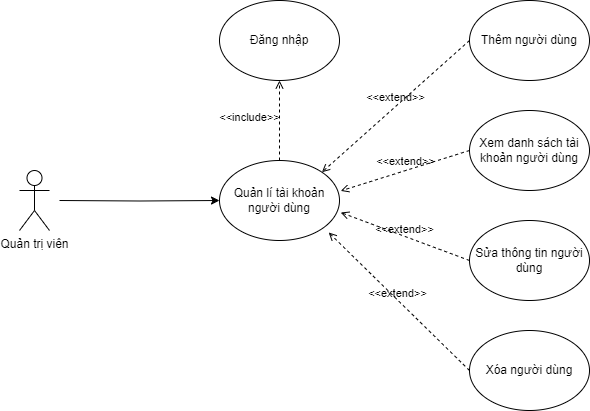
\includegraphics[width=12cm,height=13cm]{Images/use_case/use_case_manage_users.png}
    \caption[Sơ đồ use case chức năng tài khoản người dùng]{\bfseries \fontsize{12pt}{0pt}
    \selectfont Sơ đồ use case chức năng tài khoản người dùng}
    \label{use_case_user_management} %đặt tên cho ảnh
  \end{figure}

  \begin{table}[H]
    \caption{\bfseries \fontsize{12pt}{0pt}\selectfont Bảng phân tích use case chức năng xem danh sách tài khoản người dùng}
    \centering
    \begin{tabularx}{0.9\textwidth}{|c|X|}
      \hline
      \textbf{Tên chức năng} & \textbf{Xem danh sách tài khoản người dùng} \\
      \hline
      Tác nhân & Quản trị viên \\
      \hline
      Mô tả & Cho phép quản trị viên thực hiện hành động xem danh sách tài khoản người dùng \\
      \hline
      Điều kiện trước & Người dùng cần có kết nối Internet và đã đăng nhập \\
      \hline
      Dòng sự kiện chính & 
      % \begin{tabular}{@{}l@{}}
        - Quản trị viên yêu cầu xem danh sách tài khoản người dùng
        
        - Hệ thống cung cấp danh sách tài khoản người dùng

        - Quản trị viên yêu cầu một tài khoản người dùng

        - Hệ thống cung cấp thông tin tài khoản người dùng, luồng sự kiện kết thúc         
        \\
      % \end{tabular} \\
      \hline
    \end{tabularx}
  \end{table}

  \begin{table}[H]
    \caption{\bfseries \fontsize{12pt}{0pt}\selectfont Bảng phân tích use case chức năng sửa thông tin người dùng}
    \centering
    \begin{tabularx}{0.9\textwidth}{|c|X|}
      \hline
      \textbf{Tên chức năng} & \textbf{Sửa thông tin người dùng} \\
      \hline
      Tác nhân & Quản trị viên \\
      \hline
      Mô tả & Cho phép quản trị viên thực hiện hành động sửa thông tin người dùng \\
      \hline
      Điều kiện trước & Người dùng cần có kết nối Internet và đã đăng nhập \\
      \hline
      Dòng sự kiện chính & 
      % \begin{tabular}{@{}l@{}}
        - Quản trị viên yêu cầu cập nhật thông tin người dùng

        - Hệ thống hiển thị thông tin người dùng

        - Quản trị viên cung cấp thông tin cập nhật

        - Hệ thống xác minh các thông tin, nếu thỏa mãn sẽ thông báo thành công và kết thúc luồng sự kiện, ngược lại 
        sẽ thông báo lỗi         
        \\
      % \end{tabular} \\
      \hline
    \end{tabularx}
  \end{table}

  \begin{table}[H]
    \caption{\bfseries \fontsize{12pt}{0pt}\selectfont Bảng phân tích use case chức năng xóa người dùng}
    \centering
    \begin{tabularx}{0.9\textwidth}{|c|X|}
      \hline
      \textbf{Tên chức năng} & \textbf{Xóa tài khoản người dùng} \\
      \hline
      Tác nhân & Quản trị viên \\
      \hline
      Mô tả & Cho phép quản trị viên thực hiện hành động xóa tài khoản người dùng \\
      \hline
      Điều kiện trước & Người dùng cần có kết nối Internet và đã đăng nhập \\
      \hline
      Dòng sự kiện chính & 
      % \begin{tabular}{@{}l@{}}
        - Quản trị viên yêu cầu xoá một hoặc nhiều tài khoản người dùng

        - Hệ thống cung cấp thông tin người dùng cần xoá

        - Quản trị viên chọn xác nhận xóa, hệ thống xóa thông tin và gửi thông báo kết quả. Luồng sự kiện kết thúc
        \\
      % \end{tabular} \\
      \hline
    \end{tabularx}
  \end{table}

  \begin{table}[H]
    \caption{\bfseries \fontsize{12pt}{0pt}\selectfont Bảng phân tích use case chức năng quản lý đăng ký tài khoản người dùng}
    \centering
    \begin{tabularx}{0.9\textwidth}{|c|X|}
      \hline
      \textbf{Tên chức năng} & \textbf{Quản lý đăng ký tài khoản người dùng} \\
      \hline
      Tác nhân & Quản trị viên \\
      \hline
      Mô tả & Cho phép quản trị viên thực hiện hành động quản lý đăng ký đối với tài khoản người dùng \\
      \hline
      Điều kiện trước & Người dùng cần có kết nối Internet và đã đăng nhập \\
      \hline
      Dòng sự kiện chính & 
      % \begin{tabular}{@{}l@{}}
        - Quản trị viên yêu cầu xem danh sách tài khoản phê duyệt

        - Hệ thống cung cấp danh sách tài khoản phê duyệt

        - Quản trị viên yêu cầu phê duyệt một hoặc nhiều tài khoản

        - Hệ thống lưu lại thông tin tài khoản người dùng. Luồng sự kiện kết thúc        
        \\
      % \end{tabular} \\
      \hline
    \end{tabularx}
  \end{table}

\subsection{Kết luận chương}

Chương này đã thực hiện thu thập yêu cầu về
 hệ thống, nhằm tìm hiểu các mục tiêu và yêu cầu đã được đề xuất.

\newpage
